\chapter{Zero-Knowledge Proofs}
This chapter surveys selective literature about zero knowledge proofs for practical design application. The goal is to familiarize the reader with the content classification of zero-knowledge proofs in cryptography, and to give an introduction and comparison of main argument systems widely used as of today. Zero-knowledge proof systems belong to the domain of verifiable computation. Verifiable computation (VC) makes use of cryptographic protocols and arguments to verify that a computation was performed correctly. Arguments allow for false proofs only if they require very high computational power. 

The introduction of interactive proof systems (IPs) by \citet{GoldwasserIPs} and \citet{BabaiIPs} shows that only correct proofs are valid and malicious proving strategies cannot be verified. Traditional proofs are static and are made for easy, step-wise computation verification, whereas IPs require interaction between prover and verifier. In computational complexity theory, interactive proof systems are abstract machines exchanging messages between prover and verifier to convince the verifier that these sets of strings belong to a language \(L\). Here, the formal language \(L\) is defining a decision problem, i.e., a computational problem that has only two outputs, yes and no. Examples of sets of strings in \(L\) can be, that a certain Bitcoin transaction is valid, \(x = 7\) for a given \(f(x)\), or a certain object belongs to a specific merkle tree. The untrusted prover has unlimited computational power and the verifier is honest and computationally restricted. Advances in computational complexity theory during that time showed that IPs are more efficient and belong to a wider class than the traditional \textbf{NP}, i.e., problems solvable in deterministic polynomial time by reading proof strings of polynomial length \citep{SassonIOPsinproceedings}. In 1987, it was shown that every language belonging to NP has zero-knowledge proof systems \citep{anymental10.1145/28395.28420}. Later, it was shown that the class of \textbf{IP}, i.e., problems solvable by interactive proof systems, lies in \textbf{PSPACE}, i.e., problems solvable in polynomial space \citep{Shamir10.1145/146585.146609}, and that every language \(L\) in polynomial time has an interactive proof system \citep{Lund10.1145/146585.146605}. The complexity class of IP describes prover and verifier interaction in a polynomial number of rounds. Other important advances in computational complexity theory are \textbf{MIP=NEXP} \citep{Laszlo} and the \textbf{PCP theorem} \citep{PCPTheorem10.1145/278298.278306}. These works resulted in a set of proof and argument systems, that will be introduced in this chapter. \citet{Thaler} gives a further, exhaustive overview of all systems and in-depth protocol descriptions. 

The examined proof systems are secure against computationally unrestricted provers: \textit{Interactive Proof (IP), Multi-prover Interactive Proof (MIP), linear Probabilistically Checkable Proof (PCP), and Interactive Oracle Proof (IOP)}. 

Combining the systems above with cryptographic tools to force certain behavior in the proof generation will create an argument system. Argument systems are considered to be zero-knowledge, if and only if the proof does not reveal anything but its own validity \citep{GoldwasserIPs}. Adding certain properties, e.g. non-interactivity, succinctness, and knowledge, will design a certain argument of knowledge, e.g. zk-SNARK (zero-knowledge succinct non-interactive argument of knowledge). Different zk-SNARKS and notions will be examined in more detail.

The next sub chapters are structured according to the design approach described above. First, IPs, MIPs, PCPs, and IOPs will be defined. Through the combination with polynomial commitment schemes argument systems can be designed. Non-interactivity is achieved through Fiat-Shamir transformation. Second, properties and mathematical tools will be introduced to describe different arguments of knowledge: zk-SNARK, FRI-STARK and bulletproofs. Third, real-world applications of zero-knowledge proof systems will be summarized. Lastly, the different proof systems will be evaluated in different application scenarios.

\section{From Proof Systems towards Argument Systems}

A mathematical proof in the context of computer science and cryptography is any object that convinces a verifier that a statement is correct. Mathematical proofs embody what is defined in the complexity class NP. A proof system is a structured scheme that outputs a decision of whether a statement is correct or incorrect. In general, there are three properties that are desirable for proof systems \citep{GoldwasserIPs}, which will be introduced shortly. Throughout this chapter, these properties will be revisited more exhaustively.\\

\begin{center}
    \text{\parbox{420pt}{
    1. The procedure to create and verify proofs should be efficient and fast. \\
    2. \textit{Completeness}: True statements should have a convincing proof of their validity. \\
    3. \textit{Soundness}: If a statement is incorrect, there is no possibility of it having a convincing proof. \\}}
\end{center}

Unlike argument systems, proof systems do not limit the malicious prover in its computational power (\textit{statistical soundness}). Using cryptographic primitives and restricting the prover, e.g., probabilistic polynomial time proof, so that it cannot break the primitives, describes the design towards argument systems, which are computationally sound \citep{ArgSystems, MicaliArgSys}. Each proof system presented makes assumptions on the prover. However, only with the use of cryptographic tools and zero-knowledge, these proof systems can be extended with additional properties to yield zero-knowledge argument systems of various kinds.

\begin{comment}
IPs are the basis to understand cryptographic protocols and argument systems
argument systems are IP with a specific assumption
polynomial IOPs together with polynomial commitment scheme always yields a specific argument of knowledge, can be made non interactive with fiat-shamir, can be succinct too, different abwandlungen
but before we need basic understanding on different proof systems that lie behind the construction of argument systems
then we need understanding of commitment scheme and fiat shamir transform
how zero knowledge is applied in the design will be shown later when going through the different systems

information secure = only theoretically
what are those, little history
1:polynomial IOPs 
- interactive proofs intro
- MIPs
- constant round IOPs
2:linear PCPs
-intro from the book Thaler-->combined with cryptographic primitives we get SNARKs, everything is a SNARK and SNARK variation
-Luong and Park: properties intro
- Yang Yang et al properties
-Soonhyeong 2021: better verification with EVM to verify non-maliciousness of blocks (zKSNARKS used)
\end{comment}

\subsection{Interactive Proofs}

In interactive proof systems, the prover with unlimited computational resources interacts with a computationally bound verifier in order to convince the verifier of the correctness of a statement. The verifier randomly challenges the prover, which is referred to as coin tosses \citep{GoldwasserCoinTosses}. These challenges happen in rounds, until there are sufficient tests run and the verifier is convinced. \citet{GoldwasserIPs} defined an interactive proof system that is private, i.e., that the verifiers challenges are not publicly accessible, whereas the interactive proof system of \citet{BabaiIPs} allows the coin tosses to be publicly accessible by the prover.\\

    \text{\parbox{450pt}{\textbf{Interactive Proof System.} \textit{\(L\) is a language over \(\{0,1\}^n\), with n representing the input size domain of n-bit strings. An interactive protocol is a interactive proof system if after \(k\) rounds, the probabilistic verifier in polynomial time exchanged \(k\) messages with the computationally unrestricted prover, and has to either accept or decline the correctness of the prover's proposition. IP is the complexity class of problems solvable by a k-round interactive proof system.\\}}}

  
The transcript is the order in which messages are exchanged. The prover and verifier are functions \(P(x), V(x)\) with common input \(x\). The overall distribution of all transcriptions between prover and verifier is called \(View_V(P(x), V(x))\), which is bound by the number of rounds between \(P\)and \(V\). \(P\) provides a result that satisfies the proposition, e.g., \(y\) to a function \(f(x) = y\). \(P\) and \(V\) exchange a transcript of messages \((m_1, m_2, m_3, ..., m_k)\), whereby both parties take turns and the last message is sent by the prover. Note, that \(V\) is probabilistic with internal randomness \(r\). Hence, the output depends on \((V, x, r, P)\) and is \(\{0,1\}\), i.e., \(1\) if the statement is correct, and \(0\) if it is incorrect \citep{GoldwasserIPs, BabaiIPs}. Interactive proof systems have completeness error \(\delta_c\) and soundness error \(\delta_s\) . For any input \(x\), there must be a convincing proof that \(f(x)\) is correct. Incorrect statements for \(y \neq f(x)\) cannot result in a convincing proof, i.e., a malicious prover does not exist IP systems are valid if \(\delta_c, \delta_s \leq 1/3\) \citep{Thaler}.
\subsubsection{Non-interactive, publicly verifiable arguments}
The \textit{Fiat-Shamir transformation} takes any interactive proof system based on public coin tosses and transforms it into a non-interactive, publicly verifiable system. This transformation can be described effectively with the use of an ideal cryptographic assumption called \textit{Random Oracle Model (ROM)}. 
\subsubsection{Random Oracle Model}
The ROM methodology was introduced in cryptographic theory to satisfy the goal of designing secure cryptographic protocols. First, an ideal system is designed, whereby all parties have access to an oracle, i.e., a public random function. Once the security of the protocol is proven, the random oracle function is replaced by a cryptographic hashing function to implement the system in practice \citep{ROMBellare}. In IPs, the random oracle function is part of the view, i.e., random choices of challenges simulator output. It is assumed that prover and verifier can query the random oracle function \(f_R\) by sending an input \(x\), so that the random oracle returns \(f_R(x)\). In ROM, the efficiency is dependent on x, i.e., for every input in the problem size domain \(D\) , \(f_R(x)\) is captured. Since it is only practical in theory, because \(|D|\) is large to ensure security, e.g., \(2^{256}\), hash functions are used in practice \citep{ROMBellare, Thaler}, e.g., POSEIDON or SHA-3. The ROM is controversially discussed in retrospective: On the one hand, it is argued that there exist protocols that are only secure in the random oracle model and all implementation efforts in practice have led to insecure protocols, whereby the security of the ideal scheme is not maintained. The area of work at focus are digital signatures and public-key encryption, showing that the ROM is not sound \citep{ROMCanetti}. On the other hand, this conclusion is discussed to indicate there is no evidence of practical security weaknesses if there is a need for random oracle systems in a protocol. This statement is supported by protocol design examples, e.g., Elliptic Curve Digital Signature Algorithm, ECDSA, that have led to cryptographic insecurity without the use of a random oracle \citep{ROMretroKoblitz}. 
\subsubsection{Fiat-Shamir Transformation}
The Fiat-Shamir transformation \citep{ROMFiat1986HowTP} removes the need for prover-verifier interaction in a public coin interactive proof system with the help of the random oracle function. The result is a non-interactive, publicly verifiable system. IPs send messages between prover and verifier, whereby the verifier challenges the prover at random. Every message sent by the verifier in the IP is replaced by values obtained by querying the random oracle. The query always depends on the previous message sent by the prover to prevent soundness attacks. In summary, the prover only sends one message containing the transcript, i.e., the list of all messages sent by the prover and the query results of the random oracle. The input x has to be appended to the list every round. The verifier's coin tosses are not needed any longer, and there is no need for the verifier to send messages to the prover (see Figure \ref{fig:FST}).

\begin{figure}[hbt]
	\centering
		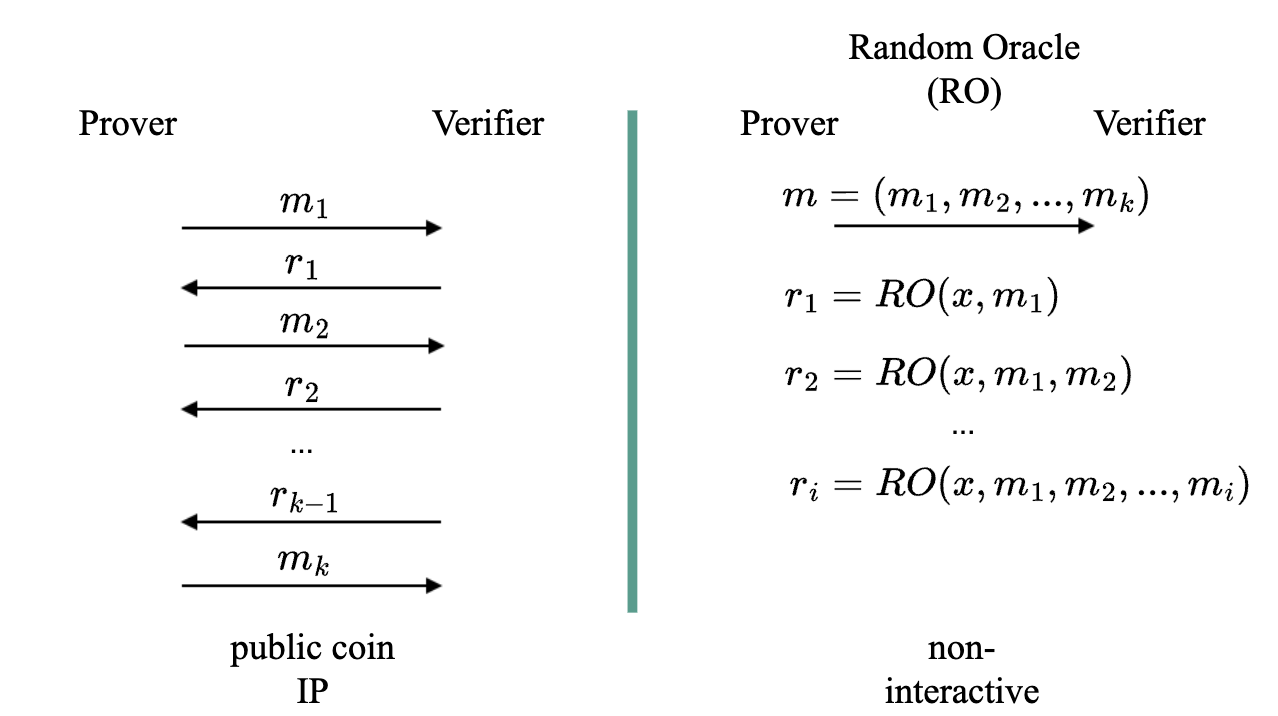
\includegraphics[width=0.8\textwidth]{Pictures/FST.png}
	\caption{Generic Fiat Shamir Transformation illustrated (based on \citet{Thaler})}
	\label{fig:FST}
\end{figure}
Argument systems are obtained by applying polynomial commitment schemes to proof systems, whereby the prover commits to a low-degree polynomial. It allows for polynomial evaluation verification without possessing all the information of this polynomial.  Polynomial commitment schemes generically are used to proof that a polynomial, evaluated at a specific input results in a specific output. The prover commits to the polynomial, which can be perceived as some object hiding the polynomial, e.g., similar to a hash. The verifier challenges the commitment with a random value. The committer then creates a proof that the polynomial evaluates at that random value at a specific point. The polynomial itself is not revealed. In interactive proof systems with an honest prover running in polynomial time, e.g., GKR protocol, any arithmetic circuit can be evaluated \citep{GKR10.1145/1374376.1374396}. Arithmetic circuits are gates that operate on two types, i.e., addition and multiplication. Retrospectively, it is an important achievement, since arbitrary computer programs can be expressed via arithmetic circuits, which is the basis layer of many zero-knowledge protocols as of today. More mathematical tools for understanding the functionality of argument systems are covered in chapter 5.2.
\begin{comment}
introduced by  GOLDWASSER, Shafi; MICALI, Silvio; RACKOFF, Charles. The
knowledge complexity of interactive proof systems. SIAM Journal
on computing. 1989, vol. 18, no. 1, pp. 186–208.
GKR protocol-->why? GKR protocol is general-purpose in the sense that it solves the problem of arithmetic circuit evaluation, and any problem in P can
be “efficiently” reduced to circuit evaluation
randomness
completeness
soundness
statistical soundness
computational soundness
fiat shamir transformation for non interactive
knowledge soundness
proof of knowledge
obtaining zero knowledge from it: verifier learns nothing about the witness
\end{comment}



\subsection{MIPs}
\subsection{Linear PCPs}
\subsection{constant round IOPs}
\subsection{Polynomial IOPs}
%(focus on chapter 10.6, combine with preliminaries from previous chapters in Thaler)

\section{Towards zero-knowledge non-interactive arguments of knowledge}


\begin{comment}
- what is zero knowledge definition
- what means indistinguishable
- different types of zero-knowledge (perfect, statistical, computational)
-first succinct argument of knowledge by goldwasser etc. 
-what is succinct
- repeat that Fiat Shamir Transformation can make them all non-interactive
-every proof from above combined with polynomial commitment schemes yields a SNARK
-short explanation what are polynomial commitment schemes: %https://coingeek.com/how-plonk-works-part-1/#:~:text=PLONK%20is%20a%20state%2Dof,by%20all%20circuits%5B1%5D.
- how: 1 design a public-coin polynomial IOP for circuit- or R1CS-satisfiability, 2 use polynomial commitment scheme 3 remove interaction via fiat shamir
- linear PCPs are exception: they need to be combined with pairing based cryptography
- everything is a sub of SNARKs
- I only want to cover three most practical zero knowledge SNARKs
- Constant-round IOPs vs. MIPs and IPs-->p.301 Thaler
- every combo with polynomial commitment scheme is a SNARK
- we focus on Groth16, PLONK, FRI-STARK, bulletproof

NITULESCU, Anca. zk-SNARKs: A Gentle Introduction [https:
/ / www . di . ens . fr / ~nitulesc / files / Survey - SNARKs . pdf].
2020. Tech. rep. ENS Paris. Accessed: 2022-05-15.
\end{comment}

\subsection{Circuit-specific zk-SNARK}
- implementation of zero-knowledge argument systems was not possible until very recently, with advances in blockchain technology
- Linear PCP and pairing based cryptography
- definitions
- R1CS, QAP and Elliptic Curve Pairing
- main functionalities: trusted setup, proof and verify
- history
- Groth16
- performance enhancements by Groth\& Maller 2017, Lipmaa 2019 and Kim Lee Oh 2020 as the newest contribution with only one single verification
- Luong and Park easy Intro
- Yang Yang et al: Intro Groth16, R1C1, QAP easy examples
- Baghery et al. mathematical backings if needed
- Benamara: ECs and pairings, good math paper 
- Guo et al: QAP, Bilinear Maps, R1CS theory



\subsection{Towards Universal Setup zk-SNARK}
PLONK is a zk-SNARK with a universal trusted set-up, which produces a structured reference string (SRS). The SRS is of size \(d\), used for circuits of up to \(\leq d\) gates. This universal SNARK has fully succinct verification and low prover run time \citep{PLONKcryptoeprint:2019/953}, compared to its predecessor Sonic \citep{SONIC10.1145/3319535.3339817}, which was the first universal and fully succinct SNARK. PLONK is based on constant round polynomial IOP and uses the polynomial commitment scheme based on \citet{Kate2010ConstantSizeCT, PLONKcryptoeprint:2019/953}. The trusted setup is universal and updateable: it can be used for the entire scheme and does not have to produced for every problem (circuit), e.g., in Groth16. Also, the Kate commitment scheme can be replaced by any other polynomial commitment scheme, e.g., FRI (see chapter 5.2.3). 
Kate commitments use the elliptic curve generated points published in the public key after trusted setup (see chapter 6.1 for detailed description) to commit to a polynomial of degree \(d\). The first \(d+1\) points are used to evaluate the polynomial at the respective coefficient. The underlying assumptions can be attributed to the \textit{Schwartz-Zippel lemma}.\\ 

    \text{\parbox{450pt}{\textbf{Schwartz-Zippel Lemma.} \textit{Let \(f(x)\) be a non-zero polynomial with degree \(d\), over \begin{math}\mathbb{F}^n\end{math}, then for a randomly chosen \(r\), the probability of \(f(r) = 0\) is at most \(\frac{d}{n}\). \\}}}
    
The \textit{Schwartz-Zippel lemma} proves that the polynomial evaluates to 0 at any point with high probability, if it evaluates to 0 at a given random \(r\). If two polynomials evaluate equally at \(r\), they are equal at every point with high probability. In a polynomial commitment scheme this suggestion is beneficial. The prover evaluates the polynomial at the random \(r\) chosen by the verifier, and sends it along with a proof. If the proof is valid, the verifier concludes that the result of the prover is also valid \citep{Kate2010ConstantSizeCT}.

The computation is first converted into an arithmetic circuit. Then, the arithmetic circuit is used to obtain a constraint system, similar to the R1CS from the previous chapter. Both have only one multiplication allowed per gate. However, PLONK only allows for one addition per gate, as long as it is not a constant. This constraint system also comes with copy constraints, which are used to transform the system into polynomials. The verification is executed using a polynomial commitment scheme (see Figure \ref{fig:plonk}).

\begin{figure}[hbt]
	\centering
		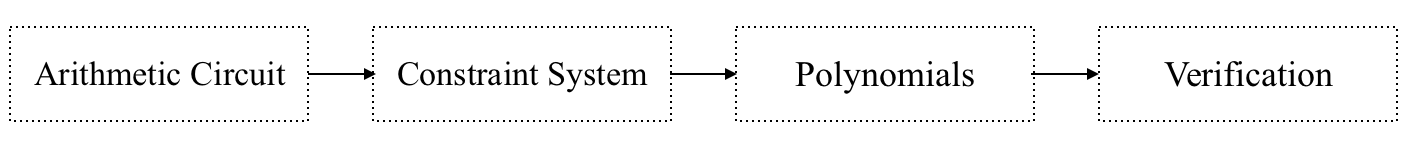
\includegraphics[width=0.8\textwidth]{Pictures/plonk_process.png}
	\caption{PLONK steps (simplified)}
	\label{fig:plonk}
\end{figure}

\begin{comment}
    PLONK
    explain CRS and SRS and why SRS is better
Constant round polynomial IOP plus Kate commitment
-definitions
-history
-plonk, it is a SNARK
-main functionality
\end{comment}

\subsection{FRI-STARK}
with FRI-based polynomial commitment
-does not use R1CS
-fri starks
-Salleras et al 2021

\subsection{Bulletproofs}
with discrete-log based polynomial commitment
- uses R1CS too
- they are non-interactive,
- they are zk arguments of knowledge
- Godden et al bulletproofs
- Chung et. al bulletproof+
- Deng at al history of bulletproofs
-Salleras et al 2021
main protocols: Lipmaa, Boudot, then Groth and Coutueau, then Hybrid from Kim Lee 2019
Deng et al 2022: history of range proofs, cuproof as example
-Kim Lee 2019: overview on range proof protocols


\section{Opportunities and Use Cases}

-e-government:e-voting/digital election

-healthcare: purchasing medical insurance contracts, patient data exchange/access
-e-auction/bidding systems
-cloud computing: zk port knocking, data deduplication, authentication schemes for cloud servers
-blockchain scaling: decrease comp cost for tx verification, zkRollups, zkSync
-querying: link traversal, zk-SQL SPARQL queries, zk based traceability systems

- Sedlmeier et al: overcoming transparency vs. privacy
- Godden et al overview of ZKP use cases: verifiable comp., linked data, identity management, access control
- ZKPs belong to verifiable computation, succinct blockchain Simunic et al 2022
- sources from Zhang et al 2021 PipeZK overview of the different Anwendungsbereiche of ZKPs-->what is verifiable outsourcing as application example?
- Maller et al 2019 Sonic: verifiable outsourcing computation example paper

\subsection{Identity Protection and Authentication}
- Bonsad et al use case
- Guo et al: e-government example
- Wang et al: hospital as trusted party, insurance receives proofs and cashes out, patient's medical data protected at all times
- Shi et al (2022): Schnorr ZKP used to proof user identity-->a bit old fashioned ZKP used maybe??
- Hunag et al 2020: good use case for MRO data sharing? zk SNARKS
- Major,Buchanan(2020): port knocking authentication scheme
- Kanagamani, Karuppiah(2021): data deduplication cloud computing with in-line block matching and ZKP properties
-Soonhyeong 2021: better verification with EVM to verify non-maliciousness of blocks (zKSNARKS used)
- Munivel Kannammal (2019): authentication scheme as additional security to prevent mobile phone password attacks on cloud storage server
- Liu Wang Peng Xing 2019: remote authentication for mobile cloud computing
-cloud computing
-egovernment, eauctions


\subsection{Data Sharing and Traceability}
- Xue and Wang: traceability use case applicable to pred. maintenance problem
-link traversal, SQL
-healthcare
-zero knowledge static program analysis: proof that a secret code is correct (Fang, Near, Darias, Zhang 2021)

\subsection{Blockchain Scaling}
- zk Roll ups, more sources needed
- Xu Chen(2021): new algorithms for zero knowledge set membership for ZK-scaling, based and compared to zkSync
- 
\section{Challenges}
- challenges can go into evaluation/comparisons of the 4 zkps
\subsection{Cost}
-Zhang et al 2021 PipeZK time and cost challenges of zKSNARK
-effieciency of ZKP: computation depends on field size-->there is a need for memory efficient ZKPs: wolverine and mac'n'cheese can do it better, but QuickSilver better protocol for large circuits (Yang, Weng, Sarkar, Wang 2021), Dittmer et al (2022) outperform Quicksilver then (most current best performing memory based protocol)
-elements from Sedlmeier Völter Strüker (2021): take the cost of Groth16

\subsection{Trust Assumption}
-Huang et al 2020 semi trusted proxy server, their assumptions
-trusted set up for zk Snarks

\subsection{Quantum Computing Threats}
1. Why are quantum verifiers a threat? (maybe Katz et al 2018)
2. different aspects of solution examples
-Deng et al 
- Xie Yang 2019: quantum secure CRS, good arguments of other shortcomings of ZKP systems, interactive and non interactive quantum zero knowledge proof systems
- Vidick Zhang 2020: describe the three problems that there are protocols developed for (big umbrella problem: quantum verification problem), good definitions from the quantum world
- also include Watrous(2009)-->coming from Vidick Zhang 2020
-Lyubashevsky et al (2020): new lattice based ZKP algorithm which is the fastest and smallest proof size for small int addition and multiplication 

\section{Evaluation Methods}
-Huang et al 2020: 1)privacy preserving and security: confidentiality, availability, integrity, privacy-preserving, traceability, single point of failure 2) performance evaluation: computing cost, number of startup nodes, privacy protection, time to generate NIZK keypair, NIZK proof, verify NIZK proof
-Zhang et al 2021 PipeZK proof generation enhancement
- Maller et al 2019 Sonic: better structured SRS in linear size to speed up proof verification

\subsection{Performance Analysis}
-Liu et al, Zheng at al: semihonest model evaluation topics-> computational complexity, communication complexity, experimental evaluation
- Liu Wang Peng Xing 2019: remote authentication for mobile cloud computing, Real-Or-Random model and BAN logic for security evaluation REGARDING different attacks
- Zhang et al 2021 PikeZK: new hardware accelerator to boost comp time for proof generation

\subsection{Sustainability}
-maybe too little literature for an own sub chapter
-Simunic et al mention need for more sustainable solutions in blockchain privacy preserving through ZKPs
-elements from Sedlmeier Völter Strüker (2021): ZKPs are more sustainable 